%!TEX root = ../Thesis.tex
\chapter{Introduction}
\label{sec:intro}
\section{Problem statement}
Many children suffer from different types of physical impairments, which significantly lowers their quality of everyday life. Cerebral palsy is most common children movement disorder, affecting on average 1.5 to 4 per 1000 infants \cite{stats}.

Cerebral palsy (CP) is a name used to describe a group of neurological disorders that affects children and has negative impact on muscle coordination and body movement \cite{main_site}. It may cause symptoms like an ataxia \footnote{\textit{ataxia} - the loss of full control of bodily movements.}, limb weakness, difficulties swallowing, speaking, making precise movements and much more. Those symptoms may vary in type and severity among individuals, depending on which parts of brain have been affected by the disease. 

CP is not curable, but rehabilitation, medication and surgeries can greatly improve both the quality of life and motor skills of the affected children. It is important to start the treatment as early as possible, so the children can enjoy nearly-normal life as adults.

The treatment, depending on symptoms and severity of the CP may consist of classic physical therapy (most important), occupational therapy, recreational therapy (improves physical and cognitive skills), speech and language therapy and more, depending on child needs. It may be combined with oral medication, used to relax stiff, contracted, or overactive muscles. Surgeries may be performed in order to help with orthopedic problems or to cut nerves to reduce chronic pain and severe spasticity.



\begin{figure}
\centering
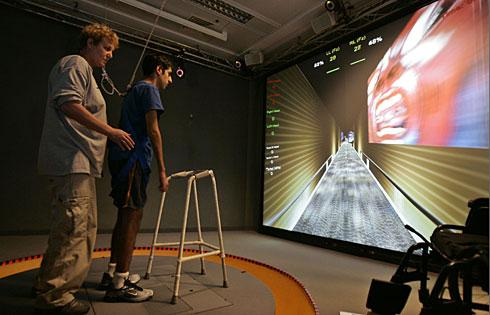
\includegraphics[width=\textwidth]{../images/rehab_example.JPG} 
\caption{Shalev Malki - disabled patient in Israel, using a virtual reality system to control a video game, that forces him to use atrophied muscles. From Chaim Sheba Medical Center, Tel Hashomer, 2006}
\label{img:example}
\end{figure}


\section{Motivation}
Different types of physical therapy are important part of supporting treatments. For some time already \cite{rehabilitation}, modern healthcare started including \emph{serious games}. \emph{Serious game} is a name for a broad genre of video games that are designed for purpose other than pure entertainment, e.g. learning, rehabilitation, information spreading. In medicine, they are used as a part of educational process \cite{exercise}, mental therapies \cite{mental_game, mental}, or rehabilitation \cite{physical_rehab, stroke_rehab}. 

Results of such experiments are promising - subjects are more willing to participate in exercises and also learn faster when enjoying the game. Enjoyment is an important factor in children rehabilitation, who often lack motivation or perseverance to perform exercise every day. 

This seems to lead to the conclusion, that serious game can be a great solution for children with cerebral palsy, who require often repeated physical rehabilitation. Creating appropriate software is not an easy problem, but greater challenge is finding appropriate control mechanism. Unfortunately, casual computer controllers - mouse, keyboard, pad - are only useful when the game focus on training cognitive skills, not physical one. The controller used in physical rehabilitation should encourage and allow movements similar to natural and not require pushing any buttons. Expensive dedicated devices could be used (e.g. Geomagic Touch\cite{phantom} - 1000\$), but for a lot of parents that's a great expense, that cannot be utilized in any other way than rehabilitation. What is important, a lot of commercial, affordable motion trackers for games and everyday computer use has been introduced in last years. Although they usually show smaller precision then dedicated devices, their availability, price and possibility of using for different applications draws a strong attention to such solution. 


\begin{figure}
\centering
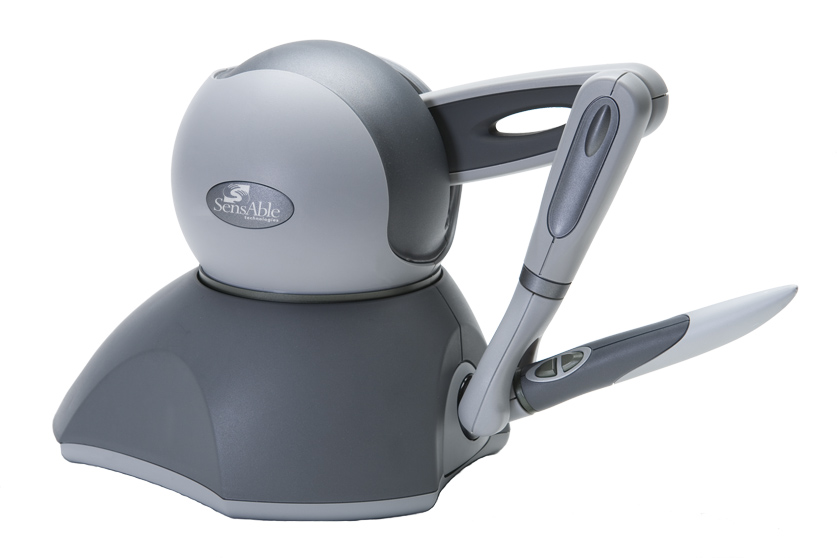
\includegraphics[width=\textwidth/2]{../images/phantom.jpg} 
\caption{Geomagic Touch - haptic device for dedicated use with modelling and medical software.}
\label{img:phantom}
\end{figure}


%rewrite the kinect 

Motion tracking is a hot topic in modern gaming. The world hype started with Microsoft Kinect \cite{Kinect} in 2010, which allowed to detected overall body movements with webcam-style technology, the industry presented more and more products with similar functionalities. Kinect was followed by PlayStation Move\cite{psmove} and Wii\cite{wiiu}, both using wand-shaped controllers for detailed motion tracking of arm movements. 

Growing crowdfunding popularity allowed smaller developers to take part in a race - that's how Sixense TrueMotion(now Razer Hydra)\cite{hydra} was funded. Other companies choose a startup path, with getting founding from large capitals, resulting in Thalmic Labs' Myo armband \cite{myo} or Leap Motion\cite{Leap} from the company of the same name. 

Using motion-tracking device could help in designing serious games for the rehabilitation, reducing the need for supervision from the therapists and also increasing the naturalness of the movements performed. 

\section{Related work}
A number of similar studies has been already performed, testing the possibility to enrich children therapy with games using different type of motion controllers:

Li et al. in their article \cite{tabletop} describe in details a process and results of designing a tabletop game for physical rehabilitation of children with CP. Important part of their study is that they worked closely with both children and therapists. Firstly, together with the therapists they identified all movements used in the rehabilitation (e.g. wrist extension, finger abduction). Then an analogue prototype was built and presented to children. Based on received feedback, the final version was implemented and tested, yielding promising results, both in opinions of therapist and children. 

During the design phase, an important problem was mentioned - compensation movements performed by child to avoid doing the desired (by therapist) ones. It is important to constrain (in hardware and software way) the possibility of such 'cheating'.

Peper et al. \cite{bimanual} presented an article about design and testing of a games for bimanual training, using new feedback method. All games were using a dedicated controller and visual (Lissajous) feedback. Three different tests were performed four times during training period, but no significant results on a group level were found. 

Bryanton et al. \cite{vr_cp} implemented and tested a VR game for ankle rehabilitation (for children with CP). The aim of this study was to check if it is possible to create a game that allows children to both train at home and strongly encourage them to do so. Only one training session took place, where both conventional and VR exercises were performed. Feedback was gathered from children, therapists and parents, who were observing the game. It was observed that children were much more excited and motivated to perform game-based exercise than normal one and seemed to be motivated to do this at home as well. Also, although number of repetition was greater in conventional exercises, range of the movement and a time of hold in maximal position was significantly larger in VR exercise, which is a encouraging result.

Luna-Olivia et al. \cite{game_xbox_360} performed the study, where they tested influence of virtual reality games controlled by low cost console on children with cerebral palsy. They used already existing games to test the theory of positive impact of playing virtual reality games on children psychomotor status. The results showed statistically significant improvement after training period, that remain even after stopping this additional exercise. 

%what did we learnerd 
%what has be done, what need to bo done
\section{Project outline}

As mentioned, recently a lot of new motion-tracking devices entered the market. Not all of them are equally popular, but some of them may be actually more successful and cheaper solutions for creating eye-hand coordination games. First, a detailed CP study should be made, with focus on which age group and CP severity level can be the best recipient of the application. Then, using factors and parameters obtained from this part, the analysis of available hardware (controllers) and software (eye and hand movement detection from video stream) will be performed to find the optimal solution.
Later, one or more prototype will be prepared, using this solutions and tested on children. The results will be evaluated to check if the analysis assumptions were correct or not. 